\documentclass[12pt,aspectratio=169]{beamer}					
\usetheme{Frankfurt}

\usecolortheme{dove}

	
\usepackage{relsize}
\usepackage[T1]{fontenc}
\usepackage[utf8]{inputenc}
\usepackage{lmodern}
						
\usepackage{xcolor}
\usepackage{amsmath}
\usepackage{mathtools}
\usepackage{amsfonts}
\usepackage{amssymb}
\usepackage{xfrac}
\usepackage[finnish, british]{babel}
\usepackage{cleveref}						
\renewcommand*\familydefault{\ttdefault} 
\usepackage{courier}
\usepackage[backend=biber,citestyle=authoryear,bibstyle=authoryear]{biblatex}
\addbibresource{references.bib}
\usepackage{csquotes} 
\usepackage[most]{tcolorbox}

\DeclareMathOperator*{\E}{\mathbb{E}}				



\graphicspath{{./plotit/}}




\useinnertheme{rectangles} 
\beamertemplatenavigationsymbolsempty	
\setbeamercovered{transparent}		 
\setbeamertemplate{frametitle}[default][colsep=-4bp,rounded=false,shadow=false] 
\definecolor{dark-gray}{gray}{0.80} 
\colorlet{lllshadecolor}{gray!15}   %for grid color


%customized colors
\definecolor{myred}{HTML}{990000}
\definecolor{myblue}{HTML}{011F5B}
\definecolor{myltblue}{HTML}{41b6e6}

\definecolor{myriver}{HTML}{D7F2FA}
\definecolor{mybackgd}{HTML}{ecf4f5}
\definecolor{klblue}{HTML}{002EA7}


\definecolor{glau}{rgb}{0.0, 0.08, 0.5}
\definecolor{cred}{rgb}{0.79, 0.0, 0.09}
\definecolor{oran}{rgb}{0.93, 0.53, 0.18}
\definecolor{dakglee}{rgb}{0, 0.42, 0.24}



\definecolor{shadecolor}{rgb}{0.98,0.98, 0.8}


\setbeamertemplate{blocks}[rounded][shadow=true]

\setbeamercolor{section in head/foot}{fg=black, bg=white}
\makeatletter

%customize background grid and logo color bar

\usepackage{tikz}                       
\usetikzlibrary{hobby,backgrounds,trees,snakes,shapes.callouts,positioning,pgfplots.groupplots}
\usetikzlibrary{positioning}
\setbeamertemplate{background}{\tikz[overlay]{
\foreach \x in {0,0.5,2,...,20} \draw[lllshadecolor,dashed](\x ,-20) -- (\x ,0);
    \foreach \y in {-20,-19.25,...,0} \draw[lllshadecolor,dashed] (0,\y) -- (20,\y);}
 
 \tikzset{every picture/.style={line width=6pt}}
 
\begin{tikzpicture}[x=1pt,y=1pt,yscale=-5,xscale=5]
\draw [color=myblue]  (0,0) -- (29,0) ;
\draw [color=myred]  (29,0) -- (58,0) ;
\draw [color=myltblue]  (58,0) -- (87,0) ;
\end{tikzpicture}

    }

   

 

\setbeamertemplate{footline}
{
  \leavevmode%
  \hbox{%
  \begin{beamercolorbox}[wd=.333333\paperwidth,ht=2.25ex,dp=1ex,center]{section in head/foot}%
    \usebeamerfont{author in head/foot}\insertshortauthor~~\beamer@ifempty{\insertshortinstitute}{}{(\insertshortinstitute)}
  \end{beamercolorbox}%
  \begin{beamercolorbox}[wd=.333333\paperwidth,ht=2.25ex,dp=1ex,center]{section in head/foot}%
    \usebeamerfont{title in head/foot}\insertshorttitle
  \end{beamercolorbox}%
  \begin{beamercolorbox}[wd=.333333\paperwidth,ht=2.25ex,dp=1ex,right]{section in head/foot}%
    \usebeamerfont{date in head/foot}%\insertshortdate{}\hspace*{2em}
    \insertframenumber{} / \inserttotalframenumber\hspace*{2ex} 
  \end{beamercolorbox}}%
  \vskip0pt%
}




\def\pdftex@driver{pdftex.def}
\ifx\Gin@driver\pdftex@driver
  \def\pgfsys@color@unstacked#1{%
    \pdfliteral{\csname\string\color@#1\endcsname}%
  }
\fi

\makeatother

\setbeamercolor{frametitle}{fg=myblue,bg=myltblue!20}



%add logo

\titlegraphic{%
  \begin{picture}(0,0)
    \put(-6,34.4){\makebox(0,0)[rt]{
\includegraphics[width=4.3cm]{logoPenn.eps}}}
    
    \put(134,33.7){\makebox(0,0)[rt]{
\includegraphics[width=1.5cm]{logoCHOP.png}}}
  \end{picture}}


\setbeamertemplate{itemize items}[circle]



\setbeamercolor{itemize item}{fg=myred}
\setbeamercolor{itemize subitem}{fg=myred}





\setbeamerfont*{block title}{family=\sffamily,series=\bfseries}



\usepackage{framed, color}
\usepackage{subcaption}
\usepackage{float} 
\usepackage{graphicx} 
\usepackage{caption} 
\usepackage{subcaption} 
\usepackage[flushleft]{threeparttable}
\usepackage{graphicx}
\usepackage[utf8]{inputenc}
\usepackage{lmodern}
\usepackage{tabularx,booktabs}
\usepackage{bbold}
\usepackage{color,colortbl}
\usepackage{bbm}
\usepackage{mathtools} 
\usepackage{amsmath,scalerel}
\usepackage{etoolbox}
\usepackage{dsfont}
\usepackage{booktabs,caption,fixltx2e}
\usepackage[flushleft]{threeparttable}
\usepackage{multirow}
\usepackage{graphicx}
\usepackage[symbol*,hang]{footmisc}
\usepackage{hyperref}
\usepackage{setspace}
\usepackage{amsmath,graphicx,centernot}

\usepackage{bbding}
\usepackage{pifont}
\usepackage{wasysym}
\usepackage{amssymb}

\usefonttheme{professionalfonts}
\usefonttheme[onlymath]{serif}


\setbeamercolor{block}{fg=mybackgd}




\usepackage{tikzmarmots}
\usepackage{etoolbox}

\setbeamercolor{block title}{use=structure,fg=black,bg=mybackgd}
\setbeamercolor{block body}{parent=normal text,use=block title,bg=mybackgd}

\setbeamercolor{block title example}{use=example text,fg=black,bg=mybackgd}
\setbeamercolor{block body example}{parent=normal text,use=block title example,bg=mybackgd}

\addtobeamertemplate{proof begin}{%
    \setbeamercolor{block title}{fg=black,bg=mybackgd}
    \setbeamercolor{block body}{fg=black, bg=mybackgd}
    \setbeamertemplate{blocks}[default]
}{}

\BeforeBeginEnvironment{theorem}{
    \setbeamercolor{block title}{fg=black,bg=mybackgd}
    \setbeamercolor{block body}{fg=black, bg=mybackgd}
}
\AfterEndEnvironment{theorem}{
 \setbeamercolor{block title}{use=structure,fg=black,bg=mybackgd}
 \setbeamercolor{block body}{parent=normal text,use=block title,bg=mybackgd, fg=black}
}

\BeforeBeginEnvironment{definition}{%
    \setbeamercolor{block title}{fg=black,bg=mybackgd}
    \setbeamercolor{block body}{fg=black, bg=mybackgd}
}
\AfterEndEnvironment{definition}{
 \setbeamercolor{block title}{use=structure,fg=black,bg=mybackgd}
 \setbeamercolor{block body}{parent=normal text,use=block title,bg=mybackgd, fg=black}
}




\title[]{Robust estimation of the causal risk difference\\ with misclassified outcome data}
\author[Shu, D]{Di Shu, PhD}
\institute[Penn\&CHOP]{Department of Biostatistics, Epidemiology and Informatics\\ University of Pennsylvania\\and\\
Center for Pediatric Clinical Effectiveness\\
 Children's Hospital of Philadelphia
}			
					  \date{September 15, 2021}

					  
					  



\usecolortheme{orchid}


\usetikzlibrary{arrows}

\usepackage{tikz}
\usetikzlibrary{positioning,arrows,shapes.geometric}

\newtcbox{\badge}[1][cred]{
  on line, 
  arc=2pt,
  colback=#1,
  colframe=#1,
  fontupper=\color{white},
  boxrule=1pt, 
  boxsep=0pt,
  left=6pt,
  right=6pt,
  top=2pt,
  bottom=2pt
}



\setbeamertemplate{mini frames}{}



\usepackage{xcolor,soul}
\definecolor{blueHL}{rgb}{.90,.95,1}



\begin{document}

\section{}
	\subsection{title}
		\begin{frame}[plain]
		
			\titlepage
		\end{frame}



	\subsection{}
		\begin{frame}{Disclosures}
			\begin{itemize}
            	
            	\item  Research to be presented was funded in part by 
            
            	\begin{itemize}
            	
            	\item The Canadian Institutes of Health Research (CIHR) Drug Safety and Effectiveness Network 
            	
       	\item The Natural Sciences and Engineering Research Council of
Canada (NSERC)

\item The Canadian Statistical Sciences Institute (CANSSI)
            		\end{itemize}
    
    
    	
            	\item All statements in this presentation are mine and do not necessarily represent the views of above funding bodies
            	
            	\item I have no conflicts of interest to disclose
            	
            	
			\end{itemize}
		\end{frame}
   
    
    \begin{frame}{Aim}
 	\setbeamercolor{whitebox}{bg=shadecolor}
  
  \begin{columns}
  \begin{column}{\paperwidth}
\begin{beamercolorbox}[sep=16pt,center]{whitebox}
  \large{To correct outcome misclassification\\ in robust estimation of the average treatment effect}
\end{beamercolorbox}
 \end{column}
  \end{columns}
\end{frame}






\begin{frame}{Outline}
 	\begin{itemize}
 	
\item Impact of outcome misclassification

\item Bias correction for 

\begin{itemize}
 	
\item inverse probability weighted (IPW) estimation


\item doubly robust (DR) estimation


\item multiply robust (MR) estimation

\end{itemize}

\end{itemize}
\end{frame}


\begin{frame}{Causal inference}
 	\begin{itemize}
\item Biomedical research often asks ${\textbf{\em causal}}$ questions
\begin{itemize}
\item Does smoking ${\textbf{\em cause}}$ lung cancer?
\item Does this new drug or vaccine ${\textbf{\em cause}}$ severe adverse reactions?
\item Does treatment A ${\textbf{\em cause}}$ more risk reduction than treatment B?

\end{itemize}
\end{itemize}
\end{frame}









\begin{frame}{Causal inference}

\begin{columns}
\begin{column}{0.5\textwidth}

 \begin{center}
   \Large  Target population
   
   \bigskip
   
   
    
     \end{center}
\end{column}
\begin{column}{0.5\textwidth}  
    \begin{center}
    \tikzset{
    woman/.pic={    
\node[transform shape, circle,fill,minimum size=4.5mm] (head) at (0,0) {};
\node[transform shape, draw, fill, trapezium, trapezium angle=55, trapezium stretches=true, rounded corners=2pt, minimum width=0.7cm, minimum height=1cm,
,below = 1pt of head, inner sep=1pt] (body) {};
\draw[transform shape, line width=1.5mm,round cap-round cap] ([shift={(-1mm,1mm)}]body.south) --++(-90:6mm);
\draw[line width=1.5mm,round cap-round cap] ([shift={(1mm,1mm)}]body.south) --++(-90:6mm);
\draw[line width=1.25mm,round cap-round cap, rounded corners] ([yshift=-.5\pgflinewidth]body.north) --++(2.5mm,0)--++(-75:6mm);
\draw[line width=1.25mm,round cap-round cap, rounded corners] ([yshift=-.5\pgflinewidth]body.north) --++(-2.5mm,0)--++(255:6mm);
}}

\begin{tikzpicture}
\foreach \i [count=\ni from 0] in {1,...,4}{
\foreach \j [count=\nj from 0] in {1,...,2}{
\pic[black!55] at (\ni,-2.5*\nj) {woman};
}}


\end{tikzpicture}
     \end{center}
\end{column}
\end{columns}
 
\end{frame}









\begin{frame}{Causal inference}

\begin{columns}
\begin{column}{0.5\textwidth}

 \begin{center}
   \Large  Target population
   
   \bigskip
   
    \badge[klblue]{Drug A}  \Large vs.  \badge[cred]{Drug B} 
    
     \end{center}
\end{column}
\begin{column}{0.5\textwidth}  %%<--- here
    \begin{center}
    \tikzset{
    woman/.pic={    
\node[transform shape, circle,fill,minimum size=4.5mm] (head) at (0,0) {};
\node[transform shape, draw, fill, trapezium, trapezium angle=55, trapezium stretches=true, rounded corners=2pt, minimum width=0.7cm, minimum height=1cm,
,below = 1pt of head, inner sep=1pt] (body) {};
\draw[transform shape, line width=1.5mm,round cap-round cap] ([shift={(-1mm,1mm)}]body.south) --++(-90:6mm);
\draw[line width=1.5mm,round cap-round cap] ([shift={(1mm,1mm)}]body.south) --++(-90:6mm);
\draw[line width=1.25mm,round cap-round cap, rounded corners] ([yshift=-.5\pgflinewidth]body.north) --++(2.5mm,0)--++(-75:6mm);
\draw[line width=1.25mm,round cap-round cap, rounded corners] ([yshift=-.5\pgflinewidth]body.north) --++(-2.5mm,0)--++(255:6mm);
}}

\begin{tikzpicture}
\foreach \i [count=\ni from 0] in {1,...,4}{
\foreach \j [count=\nj from 0] in {1,...,2}{
\pic[black!55] at (\ni,-2.5*\nj) {woman};
}}


\end{tikzpicture}
     \end{center}
\end{column}
\end{columns}
 
\end{frame}





\begin{frame}{Causal inference}
\Large For the same target population, compare

\begin{columns}
\begin{column}{0.43\textwidth}
\begin{center}
    \tikzset{
    woman/.pic={    
\node[transform shape, circle,fill,minimum size=4.5mm] (head) at (0,0) {};
\node[transform shape, draw, fill, trapezium, trapezium angle=55, trapezium stretches=true, rounded corners=2pt, minimum width=0.7cm, minimum height=1cm,
,below = 1pt of head, inner sep=1pt] (body) {};
\draw[transform shape, line width=1.5mm,round cap-round cap] ([shift={(-1mm,1mm)}]body.south) --++(-90:6mm);
\draw[line width=1.5mm,round cap-round cap] ([shift={(1mm,1mm)}]body.south) --++(-90:6mm);
\draw[line width=1.25mm,round cap-round cap, rounded corners] ([yshift=-.5\pgflinewidth]body.north) --++(2.5mm,0)--++(-75:6mm);
\draw[line width=1.25mm,round cap-round cap, rounded corners] ([yshift=-.5\pgflinewidth]body.north) --++(-2.5mm,0)--++(255:6mm);
}}

\begin{tikzpicture}
\foreach \i [count=\ni from 0] in {1,...,4}{
\foreach \j [count=\nj from 0] in {1,...,2}{
\pic[klblue] at (\ni,-2.5*\nj) {woman};
}}


\end{tikzpicture}
     \end{center}
\end{column}

\begin{column}{0.04\textwidth}  
 \begin{center}
 \Large vs.
 \end{center}
\end{column}

\begin{column}{0.43\textwidth}  
    \begin{center}
    \tikzset{
    woman/.pic={    
\node[transform shape, circle,fill,minimum size=4.5mm] (head) at (0,0) {};
\node[transform shape, draw, fill, trapezium, trapezium angle=55, trapezium stretches=true, rounded corners=2pt, minimum width=0.7cm, minimum height=1cm,
,below = 1pt of head, inner sep=1pt] (body) {};
\draw[transform shape, line width=1.5mm,round cap-round cap] ([shift={(-1mm,1mm)}]body.south) --++(-90:6mm);
\draw[line width=1.5mm,round cap-round cap] ([shift={(1mm,1mm)}]body.south) --++(-90:6mm);
\draw[line width=1.25mm,round cap-round cap, rounded corners] ([yshift=-.5\pgflinewidth]body.north) --++(2.5mm,0)--++(-75:6mm);
\draw[line width=1.25mm,round cap-round cap, rounded corners] ([yshift=-.5\pgflinewidth]body.north) --++(-2.5mm,0)--++(255:6mm);
}}

\begin{tikzpicture}
\foreach \i [count=\ni from 0] in {1,...,4}{
\foreach \j [count=\nj from 0] in {1,...,2}{
\pic[cred] at (\ni,-2.5*\nj) {woman};
}}


\end{tikzpicture}
     \end{center}
\end{column}
\end{columns}
 
\end{frame}


\begin{frame}{Effect measures for binary outcome}
 	\begin{itemize}
 
  
 \item 
 Causal risk difference or average treatment effect (ATE)

\item Causal risk ratio
\item Causal  odds ratio


\end{itemize}

\end{frame}


\begin{frame}{Effect measures for binary outcome}
 	\begin{itemize}
 
  
 \item 
 \colorbox{blue!10}{Causal risk difference or average treatment effect (ATE)}

\item Causal risk ratio
\item Causal  odds ratio


\end{itemize}

\end{frame}





\begin{frame}{Motivating example: smoking cessation data}


 
\begin{itemize}
\item  Data structure

\begin{itemize}
\item $X$: a vector of baseline covariates

\item $T$:  treatment

\item $Y$: smoking cessation status 

\end{itemize}

\item \colorbox{blue!10}{Objective}:  To estimate  {\color{cred} $\tau_0=E\{Y(1)\}-E\{Y(0)\}$}, where

\begin{itemize}
\item
$Y(1)$:  potential outcome that would have been observed had the  individual been treated


\item

$Y(0)$: potential outcome that would have been observed had the  individual been untreated

\item $\tau_0$ is the {\color{cred} causal risk difference}
\end{itemize}


\end{itemize}

\end{frame}




\begin{frame}{Motivating example: causal interpretation}
  \begin{itemize}
 
 \item
$E\{Y(1)\}$:  smoking cessation rate that would have been observed had the entire population been treated


\item
$E\{Y(0)\}$: smoking cessation rate that would have been observed had the entire population been untreated


\item

Causal effect $\tau_0=E\{Y(1)\}-E\{Y(0)\}$ compares  outcomes in two hypothetical worlds (treatment vs. control) for {\color{cred}  the same entire population} 

  \end{itemize}
\end{frame}







\begin{frame}{Motivating example: challenge}
 \begin{itemize}
\item Outcome of interest: smoking cessation status 
 
\item Collected data:  {\color{cred} self-reported} smoking cessation status using
\begin{itemize}
\item phone interview (e.g. Lee et al. 2013)
\item  self-administrated online  survey

\end{itemize}


\item {\color{cred} No biochemical verification} of cessation status


\item Some smokers might report that they had quit smoking

\begin{itemize}
\item outcomes data are subject to misclassification
\item the true outcome {\color{cred}  $Y$ is unobserved }
\end{itemize}
\end{itemize}
  \vfill
{\color{black!40}{\scriptsize Lee SM, Landry J, Jones PM, Buhrmann O, Morley-Forster P. The effectiveness of a perioperative smoking cessation program: a randomized clinical trial. Anesth Analg 2013;117(3):605-13.}}
\end{frame}




\begin{frame}{Inverse probability weighted (IPW) estimation}

\begin{itemize}

\item Let $e=P(T=1|X)$ be the propensity score (Rosenbaum and Rubin 1983)

\item IPW estimator:
\[
\hat\tau=n^{-1}\sum_{i=1}^n \dfrac{T_i{\color{cred}Y_i}}{\hat{e}_i}-n^{-1}\sum_{i=1}^n \dfrac{(1-T_i){\color{cred}Y_i}}{1-\hat{e}_i}
\]
  


\pause 
\item
$Y_i$ is unobserved in the presence of misclassification

\item Let $Y_i^\ast$ denote the observed outcome and $\hat\tau^\ast$ the naive estimator

\end{itemize}

  \vfill
{\color{black!40}{\scriptsize Rosenbaum PR, Rubin DB. The central role of the propensity score in observational studies for causal effects. Biometrika 1983;70(1):41-55.}}
\end{frame}




\begin{frame}{Why misclassification matters}
\begin{itemize}
\item
Let ${\color{cred}p_{ab}}=P(Y^\ast=a|Y=b)$ for $a, b=0, 1$
 
\begin{itemize}
\item $p_{11}$: sensitivity
\item $p_{00}$: specificity
\item $p_{10}+p_{01}$: \text{total error}
\end{itemize}

\end{itemize}

\begin{block}
\noindent {\bf {\color{glau}Theorem 1a (Shu and Yi 2019)}}:
{\it

\begin{itemize}

\item  Naive estimator {\color{cred}$\hat\tau^\ast\rightarrow (p_{11}-p_{10}) \tau_0$} in probability as $n\rightarrow  \infty$

\item Asymptotic  {\color{cred} bias} of the naive estimator {\color{cred}is
$
-\text{total error}\times \tau_0
$}

\item Asymptotic  {\color{cred}relative bias  is
$
-\text{total error}
$
}

\end{itemize}
}
\end{block}

 \vfill
{\color{black!40}{\scriptsize Shu D, Yi GY. Causal inference with measurement error in outcomes: bias analysis and estimation methods. Stat Methods Med Res 2019;28(7):2049-68.}}
\end{frame}






\begin{frame}{Closed-form bias correction}

\begin{block}
\noindent {\bf {\color{glau}Theorem 1b (Shu and Yi 2019)}}:
{\it

\begin{itemize}


\item  {\color{cred}Propose}  $\hat\tau=\dfrac{\hat\tau^\ast}{p_{11}-p_{10}}=\dfrac{\text{naive}}{1-\text{total error}}=\dfrac{\text{naive}}{\text{sens}+\text{spec}-1}$

\item
$\hat\tau$ is {\color{cred}consistent} :  {\color{cred}$\hat\tau\rightarrow  \tau_0$} in probability as $n\rightarrow  \infty$

\end{itemize}
}
\end{block}

\bigskip

\begin{itemize}

\item Remark 1: \colorbox{blue!10}{attenuation effect} of outcome misclassification

\pause

\item Remark 2: we can specify or estimate $p_{ab}$ using additional info and data (e.g. validation sample, repeated measures)

\item Remark 3: extension that allows for more complicated misclassification model (i.e. $Y^\ast$ depends on $Y$, $T$ and/or $X$) is available


\end{itemize}
\end{frame}






\begin{frame}{Selected simulation results}

{\small Performance of  the corrected estimator $\hat\tau$  in comparison to the naive estimator $\hat\tau^\ast$ with 5000 simulation runs; ReBias$(\%)$: average relative bias; CP$(\%)$:  coverage percentage}

\begin{table}[t]
\tabcolsep7pt
\begin{center}
\begin{tabular}{rrrrrrrrrrrrrrr}
\toprule
  setting    && \multicolumn{2}{c}{$n=1000$} &\multicolumn{3}{c}{$n=5000$}\\
\cline{3-4}     \cline{6-7} \\
$p_{11}=p_{00}$    &Method  & ReBias$(\%)$  &CP$(\%)$&& ReBias$(\%)$  &CP$(\%)$   \\ 
  \hline
$0.9$&Naive  & -19.6   &82.7&&-19.8    &35.1 \\
\vspace{2mm}

\cellcolor{blueHL}
&\cellcolor{blueHL}Corrected & \cellcolor{blueHL}0.6    &\cellcolor{blueHL}95.1& \cellcolor{blueHL} &\cellcolor{blueHL} 0.2 &\cellcolor{blueHL} 95.4  \\
$0.8$&Naive     &-39.7& 46.5 &   & -40.1  &0.50 \\
\vspace{2mm}

\cellcolor{blueHL}
&\cellcolor{blueHL}Corrected &  \cellcolor{blueHL}0.5   &\cellcolor{blueHL}95.3& \cellcolor{blueHL}&  \cellcolor{blueHL}-0.2& \cellcolor{blueHL}94.7  \\
$0.7$&Naive     &-60.3     &13.9&& -60.0   &0.00\\
 
 \cellcolor{blueHL}
&\cellcolor{blueHL}Corrected  & \cellcolor{blueHL}-0.7  &\cellcolor{blueHL}94.6&\cellcolor{blueHL}& \cellcolor{blueHL}0.1  &\cellcolor{blueHL}94.6  \\
\bottomrule
\end{tabular}
\end{center}
\end{table}

\end{frame}






\begin{frame}{Real-world application}
\begin{itemize}
\item Evaluation of a perioperative smoking cessation program (Lee et al. 2013)


\item 

\underline{{\color{blue}Outcome of interest}}: smoking cessation status for previous 7 days at the 30-day follow-up {\color{dakglee}postoperatively}

\item

$Y=1$ if no smoking, $Y=0$ if still smoking

\item

\underline{{\color{blue}Outcome collected}}: {\color{cred}self-reported} smoking cessation status  answered on the phone, {\color{cred}without verification}

\pause

\item

Reasonable to assume $p_{11}=1$

\item

\underline{{\color{blue}Misclassification}}: {\color{dakglee}preoperative} self-reported outcomes  confirmed by  exhaled CO levels  $\rightarrow \text{specify}\,\,  p_{10}=0.075$


\item

\underline{{\color{blue}Analysis}}: $\hat\tau^\ast=0.170$, $\hat\tau=\dfrac{\hat\tau^\ast}{p_{11}-p_{10}}=\dfrac{0.170}{1-0.075}=0.184$

\end{itemize}
\end{frame}





\begin{frame}{Double robustness}

\begin{itemize}
\item 
The validity of IPW estimators  requires propensity score model be  correctly specified 

\item Doubly robust (DR) estimators provide more {\color{cred}protection against model misspecification} (e.g. Robins et al. 1994, Lunceford and Davidian 2004) by simultaneously using
\begin{itemize}
\item A propensity score model
\item An outcome model
\end{itemize}
\end{itemize}
\vfill
{\color{black!40}{\scriptsize Robins JM, Rotnitzky A, Zhao LP. Estimation of regression coefficients when some regressors are not always observed. Am Stat Assoc 1994;89(427):846-66.}}

{\color{black!40}{\scriptsize Lunceford JK, Davidian M. Stratification and weighting via the propensity score in estimation of causal treatment effects: a comparative study. Stat Med 2004;23(19):2937-60.}}

\end{frame}







\begin{frame}{Correcting outcome misclassification}

\begin{itemize}

 \item
 A  {\color{cred}bias-corrected} DR estimator:
 \[
{\color{cred}\hat\tau_{DR}}=\hat E(Y_1)-\hat E(Y_0),\,\,\text{where}
\]
{\small
\[
\hat E(Y_1)=\dfrac{1}{n}\sum_{i=1}^n \left\{\dfrac{T_iY_i^\ast}{\hat e_i(p_{11}-p_{10})}-\dfrac{T_i-\hat e_i}{\hat e_i}\hat q_{i1}-\dfrac{T_i}{\hat e_i}\left(\dfrac{p_{10}}{p_{11}-p_{10}}\right)\right\}
\]
\[
\hat E(Y_0)=\dfrac{1}{n}\sum_{i=1}^n \left\{\dfrac{(1-T_i)Y_i^\ast}{(1-\hat e_i)(p_{11}-p_{10})}+\dfrac{T_i-\hat e_i}{1-\hat e_i}\hat q_{i0}-\dfrac{1-T_i}{1-\hat e_i}\left(\dfrac{p_{10}}{p_{11}-p_{10}}\right)\right\}
\]
}
 $\hat q_{i1}$ is an estimate of $P(Y_i=1|T_i=1, X_i)$ and  $\hat q_{i0}$ is an estimate of $P(Y_i=1|T_i=0, X_i)$


\end{itemize}

\end{frame}


\begin{frame}{Correcting outcome misclassification}

\begin{itemize}
\item  $\hat q_{i1}$ and $\hat q_{i0}$ cannot be calculated by  fitting the postulated outcome model,  because the true value $Y$ is unobserved

\item Maximize the observed likelihood instead



\pause


\bigskip

\item Let $\boldsymbol\beta$ be the  outcome model parameters

 \item {\color{cred}Observed likelihood} function contributed from subject $i$:
\begin{eqnarray*}
 L_i(\boldsymbol\beta)&=&P(Y_i=1|T_i, X_i; \boldsymbol\beta)\{p_{11}Y_i^\ast+(1-p_{11})(1-Y_i^\ast)\}\\
 &&+P(Y_i=0|T_i, X_i; \boldsymbol\beta)\{p_{10}Y_i^\ast+(1-p_{10})(1-Y_i^\ast)\}
\end{eqnarray*}

\end{itemize}


\end{frame}






\begin{frame}{Correcting outcome misclassification}


\begin{block}
\noindent {\bf {\color{glau}Theorem 2 (Shu and Yi 2019)}}:
{\it
The proposed estimator $\hat\tau_{DR}$ is {\color{cred}doubly robust}, i.e., it is  {\color{cred}consistent}  when either the propensity score model $T\sim X$ or the outcome model $Y\sim (X, T)$ is correctly specified.
}
\end{block}

\bigskip

\begin{itemize}

\item Remark: extension that allows for more complicated misclassification model (i.e. $Y^\ast$ depends on $Y$, $T$ and/or $X$) is available


\end{itemize}

\end{frame}






\begin{frame}{Selected simulation results}

{\small Performance of  the DR estimator $\hat\tau_{DR}$  with 5000 simulation runs; \\
Scenario: whether the treatment and outcome models are correct or not}

\begin{table}[t]
\tabcolsep10pt
\begin{center}
\begin{tabular}{rrrrrrrrrrrrr}
\toprule
 &     & \multicolumn{3}{c}{$p_{11}=0.9, \,\,p_{10}=0.1$} &\multicolumn{2}{c}{$p_{11}=0.8, \,\,p_{10}=0.2$}\\
\cline{3-4}     \cline{6-7} \\
$n$  &Scenario  & ReBias$(\%)$    & CP$\%$&&  ReBias$(\%)$    & CP$\%$ \\\midrule
2000 & {\color{glau}\ding{52}} {\color{glau}\ding{52}}& 0.0&95.1&&-0.9 &94.2\\
&{\color{glau}\ding{52}} {\color{cred}\ding{56}}&-0.9 &95.0&&0.5 & 93.5 \\
\vspace{3mm}
&{\color{cred}\ding{56}} {\color{glau}\ding{52}}& 0.1 &96.4&&0.9& 94.4 \\

5000&{\color{glau}\ding{52}} {\color{glau}\ding{52}}&0.1&  95.5&&-0.4&94.8\\
&{\color{glau}\ding{52}} {\color{cred}\ding{56}}&1.0&96.1&&0.3 & 95.1 \\
&{\color{cred}\ding{56}} {\color{glau}\ding{52}}& 0.3 &95.4&&0.3&96.0 \\
\bottomrule
\end{tabular}
\end{center}
\end{table}

\end{frame}




\begin{frame}{Multiple robustness}
 \begin{itemize}
 \item What if both the treatment and outcome models are wrong?
 
 \pause
 
 \bigskip
 
 \item Han and Wang (2013) developed a {\color{cred}multiply robust (MR)} method by simultaneously using
\begin{itemize}
\item {\color{cred}A set of}   propensity score models
\item {\color{cred}A set of}   outcome models
\end{itemize}

 
 \item Only one model needs to be correct
 

 \end{itemize}
  \vfill
{\color{black!40}{\scriptsize Han P, Wang L. Estimation with missing data: beyond double robustness. Biometrika 2013;100(2):417-30.}}
\end{frame}




\begin{frame}{Specifying two model sets}
\begin{itemize}
\item Let $e(X)=P(T=1|X)$ be the true treatment  model  and  $q_t(X)=P(Y=1|X, T=t)$ the true outcome model




\item Individuals $i=1,\ldots,m$ are treated, $i=m+1,\ldots,n$ are untreated

\bigskip

\item Postulate
\begin{itemize}
\item ${\color{cred}\mathcal{E}}=\{e^j(\boldsymbol\gamma^j; X),j=1\ldots,J\}$:  a set of $J$  {\color{cred}treatment} models

\item ${\color{cred}\mathcal{Q}}=\{q_t^k(\boldsymbol\beta^k; X),k=1\ldots,K\}$: a set of $K$ {\color{cred} outcome} models

\end{itemize}




\end{itemize}
\end{frame}




\begin{frame}{MR estimation without misclassification}
\begin{itemize}


\item  Applying the method of Han and Wang (2013):

\begin{itemize}
\item 

Step 1: obtain $\hat{\boldsymbol\gamma}^j$ by fitting the $j$th treatment model, for each $j$

\item {Step 2}: obtain $\hat{\boldsymbol\beta}^k$ by fitting the $k$th {outcome} model, for each $k$

\item Step 3: calculate  $\hat w_i$  and  $\tilde w_i$ [that use $\hat{\boldsymbol\gamma}^j$ and $\hat{\boldsymbol\beta}^k$]

\item {Step 4}:  calculate


\[
\,\, \hat E(Y_1)=\sum_{i=1}^m \hat w_iY_i
\,\,\,\,
\text{and}
\,\,\,\,
\hat E(Y_0)=\sum_{i=m+1}^{n}  \tilde w_i Y_i
\]

\item Step 5:  calculate $\hat\tau=\hat E(Y_1)-\hat E(Y_0)$

\end{itemize}


\end{itemize}

\end{frame}









\begin{frame}{MR estimation without misclassification}
\begin{itemize}



\item Define 

\begin{itemize}
\item

$\hat\theta^j=n^{-1}\sum_{i=1}^n e^j(\hat{\boldsymbol\gamma}^j; X_i)$ for $j=1,\ldots,J$

 \item  $\hat\eta_1^k=n^{-1}\sum_{i=1}^n q_1^k(\hat{\boldsymbol\beta}^k; X_i)$ and $\hat\eta_0^k=n^{-1}\sum_{i=1}^n q_0^k(\hat{\boldsymbol\beta}^k; X_i)$ for $k=1,\ldots,K$ 


\end{itemize}



\item
$
\hat w_i=\left\{\dfrac{1}{m}\dfrac{1}{1+\hat\rho^T \hat g_i(\hat{\boldsymbol\gamma},\hat{\boldsymbol\beta}) }\right\}\bigg/\left\{\dfrac{1}{m}\sum_{i=1}^m\dfrac{1}{1+\hat\rho^T \hat g_i(\hat{\boldsymbol\gamma},\hat{\boldsymbol\beta}) }\right\}
$

\begin{itemize}

\item  $\hat\rho$ solves $\sum_{i=1}^m{\hat g_i(\hat{\boldsymbol\gamma},\hat{\boldsymbol\beta})}/\{1+\rho^T  \hat g_i(\hat{\boldsymbol\gamma},\hat{\boldsymbol\beta})\}=\boldsymbol 0$ for $\rho$, with
{\small
$
\hat g_i(\hat{\boldsymbol\gamma},\hat{\boldsymbol\beta})=(e^1(\hat{\boldsymbol\gamma}^1; X_i)-\hat\theta^1,\ldots, e^J(\hat{\boldsymbol\gamma}^J; X_i)-\hat\theta^J, q_1^1(\hat{\boldsymbol\beta}^1; X_i)-\hat\eta_1^1,\ldots, q_1^K(\hat{\boldsymbol\beta}^K; X_i)-\hat\eta_1^K)^T 
$ 
}
\end{itemize}


\bigskip
\item Calculate $\tilde w_i$ similarly

\end{itemize}

\end{frame}









\begin{frame}{MR estimation without misclassification}
\begin{itemize}


\item  Applying the method of Han and Wang (2013):

\begin{itemize}
\item 

Step 1: obtain $\hat{\boldsymbol\gamma}^j$ by fitting the $j$th treatment model, for each $j$

\item \colorbox{blue!10}{Step 2}: obtain $\hat{\boldsymbol\beta}^k$ by fitting the $k$th \colorbox{blue!10}{outcome} model, for each $k$

\item Step 3: calculate  $\hat w_i$  and  $\tilde w_i$ [that use $\hat{\boldsymbol\gamma}^j$ and $\hat{\boldsymbol\beta}^k$]

\item \colorbox{blue!10}{Step 4}:  calculate


\[
\,\, \hat E(Y_1)=\sum_{i=1}^m \hat w_i{\color{cred}Y_i}
\,\,\,\,
\text{and}
\,\,\,\,
\hat E(Y_0)=\sum_{i=m+1}^{n}  \tilde w_i {\color{cred}Y_i}
\]

\item Step 5:  calculate $\hat\tau=\hat E(Y_1)-\hat E(Y_0)$

\end{itemize}


\end{itemize}

\end{frame}





\begin{frame}{MR estimation with  outcome misclassification}
\begin{itemize}
\item 

{\color{cred}Misclassification}: $p_{ab}=P(Y^\ast=a|Y=b)$  for $a, b=0, 1$.



\item Correction method (Shu and Yi 2021 submitted)

\begin{itemize}
\item 

Step 1: obtain $\hat{\boldsymbol\gamma}^j$ by fitting the $j$th treatment model,  for each $j$

\item \colorbox{blue!10}{Step 2}: obtain $\hat{\boldsymbol\beta}^k$ by maximizing the {\color{cred}observed} likelihood,  for each $k$ 

\item Step 3: calculate  $\hat w_i$  and  $\tilde w_i$

\item \colorbox{blue!10}{Step 4}:  calculate
$
\,\, \hat E(Y_1)=\sum_{i=1}^m \dfrac {\hat w_iY_i^\ast}{{\color{cred}p_{11}-p_{10}}}-{\color{cred}\dfrac{p_{10}}{p_{11}-p_{10}}}
$
\[
\hat E(Y_0)=\sum_{i=m+1}^{n}   \dfrac {\tilde w_i Y_i^\ast}{{\color{cred} p_{11}-p_{10}}}-{\color{cred}\dfrac{p_{10}}{p_{11}-p_{10}}}
\]

\item Step 5:  calculate $\hat\tau_{MR}=\hat E(Y_1)-\hat E(Y_0)$

\end{itemize}


\end{itemize}

\end{frame}





\begin{frame}{MR estimation with  outcome misclassification}


\begin{block}
\noindent {\bf {\color{glau}Theorem 3 (Shu and Yi 2021 submitted)}}:
{\it
The proposed estimator $\hat\tau_{MR}$ is {\color{cred}multiply robust}, i.e., it is {\color{cred}consistent} when either {\color{cred}$\mathcal{E}$ or $\mathcal{Q}$ contains a correctly} specified model.
}
\end{block}


 \vfill
{\color{black!40}{\scriptsize Shu D, Yi GY. Multiply robust estimation of causal treatment effects with binary outcome data subject to misclassification. Submitted.}}
\end{frame}






\begin{frame}{Selected simulation results}

{\small Performance of  the MR estimator $\hat\tau_{MR}$  with 5000 simulation runs when $(p_{11},p_{10})=(0.7,0.3)$; 
Scenarios I or II: only the treatment model set or only the outcome model set contains a correct model}

\begin{table}[t]
\tabcolsep8pt
\begin{center}
\begin{tabular}{rrrrrrrrrrrrrrrrrrrrrrr}
\toprule
     && \multicolumn{3}{c}{$n=2000$} &\multicolumn{2}{c}{$n=5000$}\\
\cline{3-4}     \cline{6-7} \\
Scenario &Method  & ReBias$\%$    & CP$\%$&&  ReBias$\%$    & CP$\%$ \\\midrule
I&Naive&-59.76&1.50&&-60.39&0.1\\
\vspace{2mm}
\cellcolor{blueHL} &\cellcolor{blueHL}  $\hat\tau_{MR}$& \cellcolor{blueHL} 0.64& \cellcolor{blueHL} 93.6& \cellcolor{blueHL} & \cellcolor{blueHL} -0.90& \cellcolor{blueHL} 93.7&\cellcolor{blueHL}\\
II&Naive&-60.32&1.50&&-60.47&0.0\\
\vspace{2mm}
\cellcolor{blueHL} &\cellcolor{blueHL} $\hat\tau_{MR}$& \cellcolor{blueHL} -0.48& \cellcolor{blueHL} 94.9& \cellcolor{blueHL} & \cellcolor{blueHL} -0.59&\cellcolor{blueHL}  94.2&\cellcolor{blueHL}\\
\bottomrule
\end{tabular}

\end{center}
\end{table}

\end{frame}



  


\begin{frame}{Smoking cessation data revisited}

 \begin{itemize}

\item

\underline{{\color{blue}Naive}}: $\hat\tau^\ast=0.170\,\, (\text{CI}\,\, 0.041, 0.307)$

\bigskip

\item Reasonable to assume $p_{11}=1$

\item

\underline{{\color{blue}Misclassification}}: use {\color{dakglee}preoperative} data $\rightarrow \text{specify}\,\,  p_{10}=0.075$





\item

\underline{{\color{blue}Corrected}}:
$\hat\tau_{MR}=0.189\,\, (\text{CI}\,\, 0.051, 0.324)$

\end{itemize}

\end{frame}



\begin{frame}{Smoking cessation data revisited}

    \begin{center}
     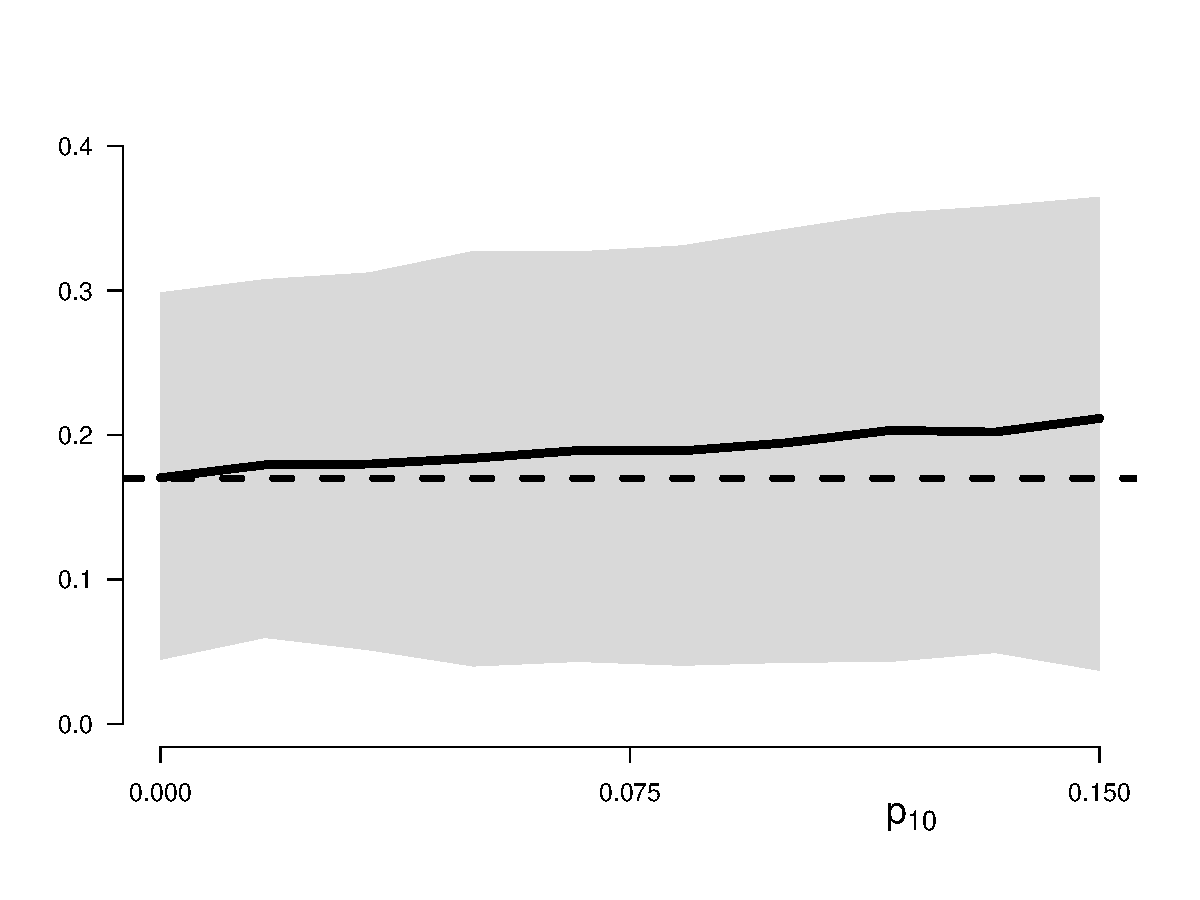
\includegraphics[width=0.5\textwidth]{MRplot.pdf}
     \end{center}
 
{\small Sensitivity analysis with $p_{10}$ ranging from 0 to 0.15. Solid line: point estimates; Grey region:  bootstrap percentile 95\% CIs. Dashed line: naive estimate (i.e. 0.170)}
\end{frame}




\begin{frame}{Outcome misclassification + X}
  \begin{center}
     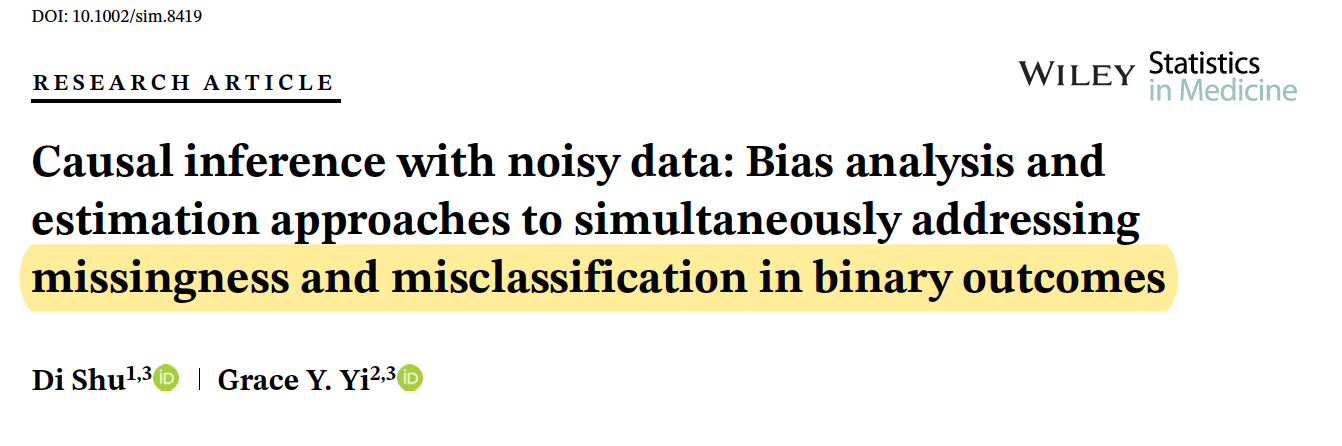
\includegraphics[width=0.6\textwidth]{ext1.png}
    
       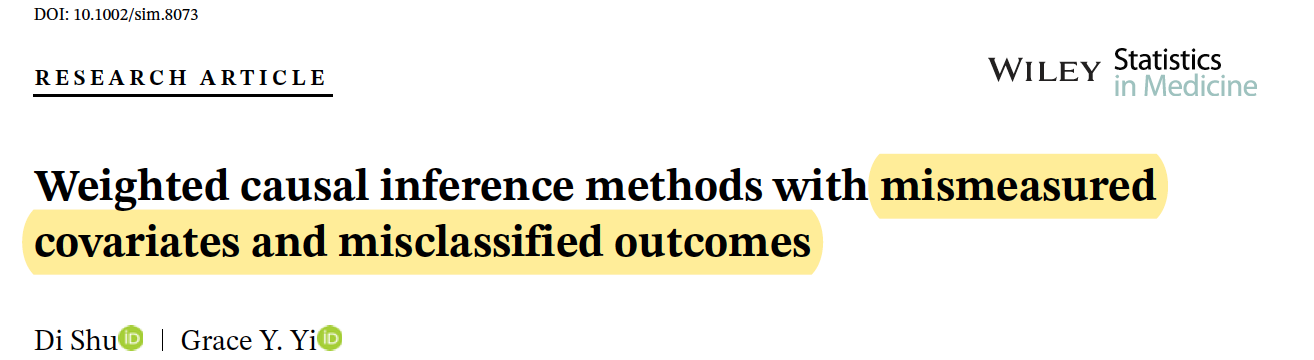
\includegraphics[width=0.6\textwidth]{ext2.png}
     \end{center}
\end{frame}




\begin{frame}{Future topics}
 \begin{center}
     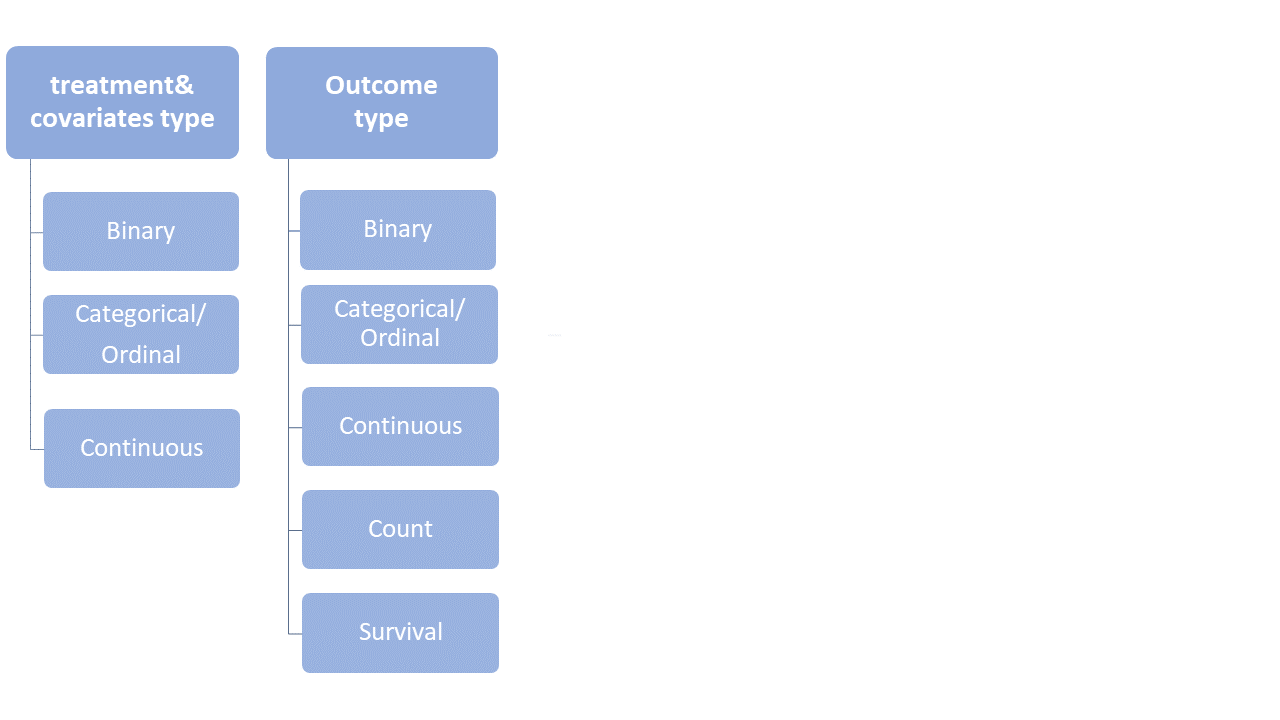
\includegraphics[width=0.85\textwidth]{fi1.png}
     \end{center}
\end{frame}


\begin{frame}{Future topics}
 \begin{center}
     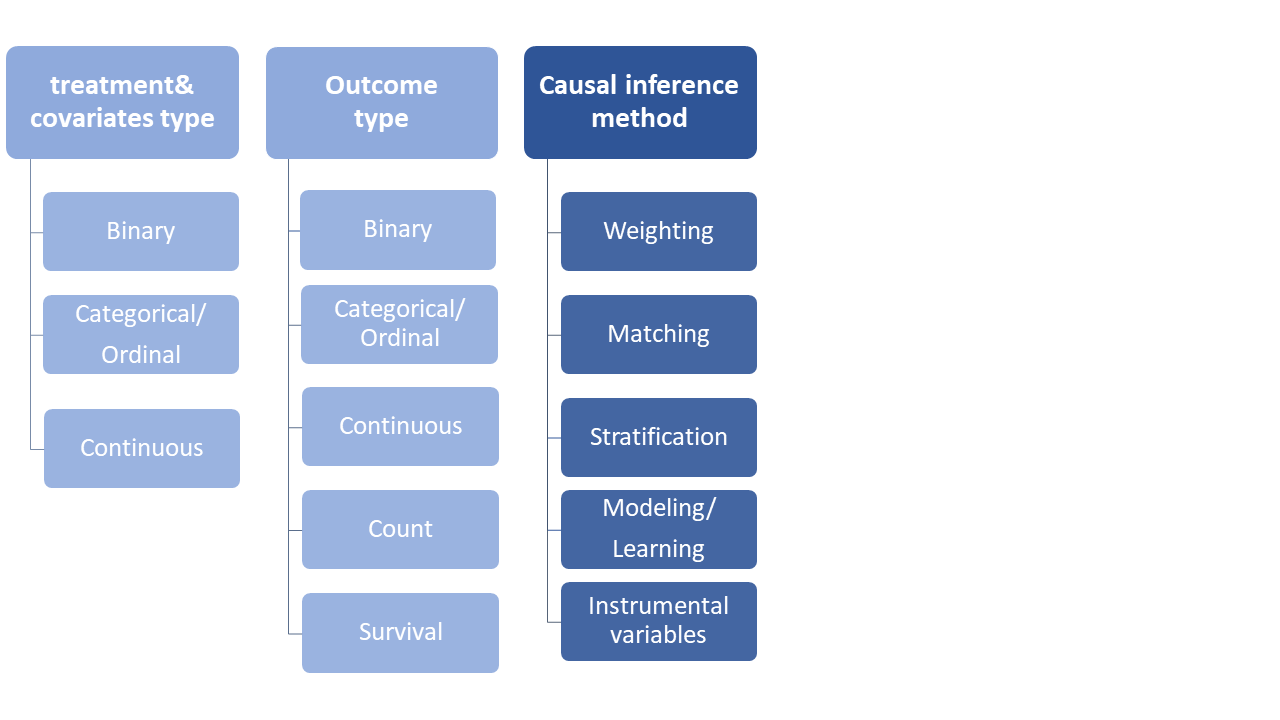
\includegraphics[width=0.85\textwidth]{fi2.png}
     \end{center}
\end{frame}

\begin{frame}{Future topics}
 \begin{center}
     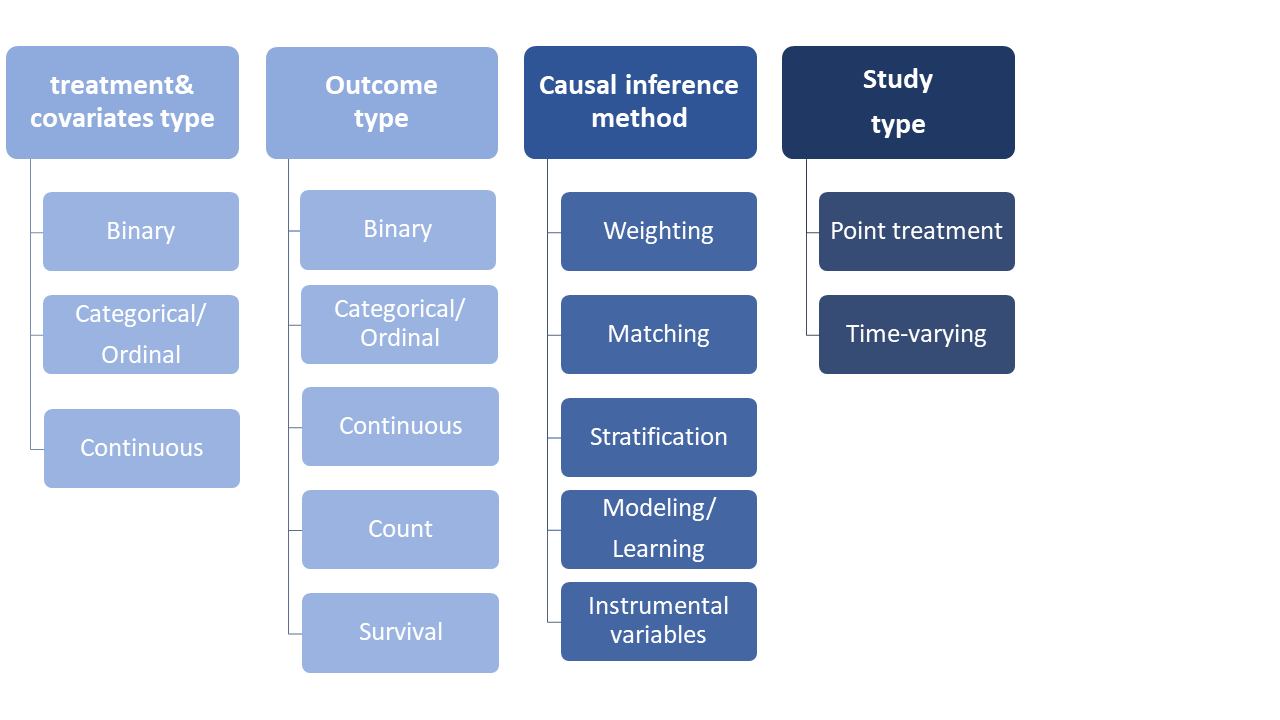
\includegraphics[width=0.85\textwidth]{fi3.png}
     \end{center}
\end{frame}


\begin{frame}{Future topics}
 \begin{center}
     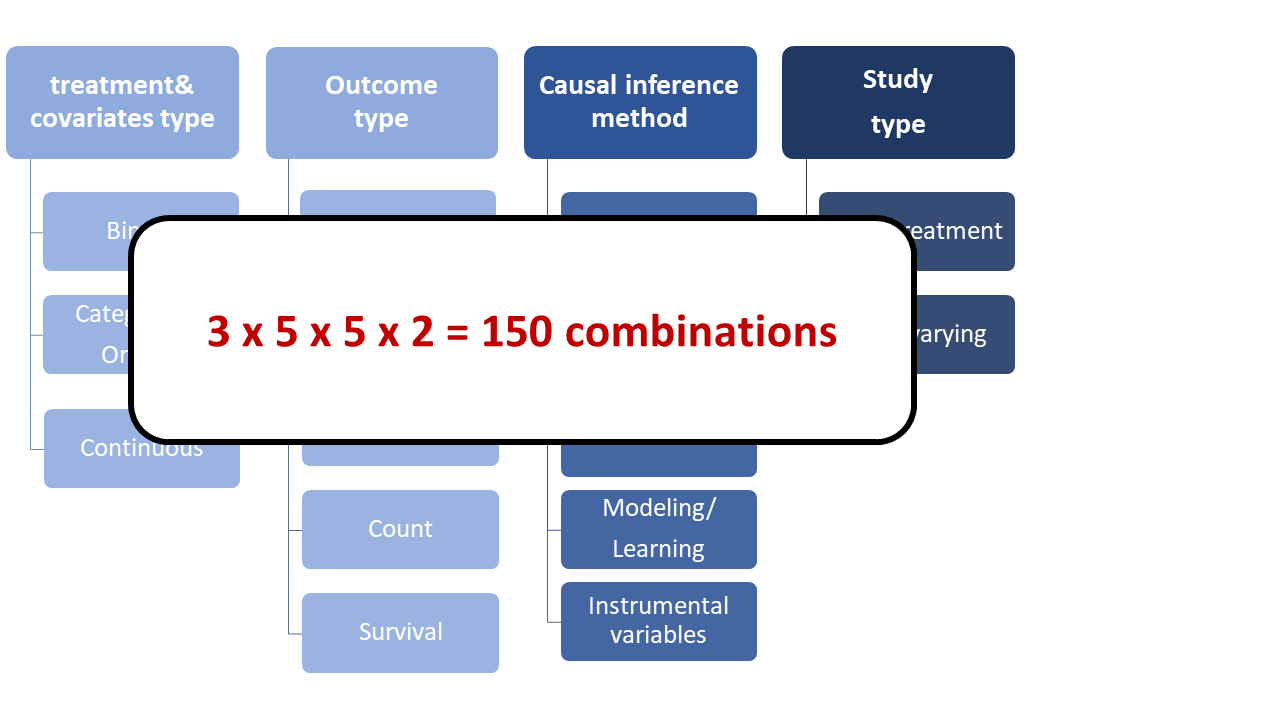
\includegraphics[width=0.85\textwidth]{fi4.png}
     \end{center}
\end{frame}





\begin{frame}{Acknowledgement}
 Joint work with Dr. Grace Yi,  University of Western Ontario
\end{frame}




\begin{frame}{Thank you!}
 \begin{center}
 
 \Large{\color{myblue}{\textbf{Di.Shu@pennmedicine.upenn.edu}}}
 
 \end{center}
\end{frame}








\end{document}